%% Article SC-Reborn pour International Journal of Production Economics
%% MATÉRIEL SUPPLÉMENTAIRE : compléments retirés du manuscrit principal (manuscrit.tex).
%% Les renvois « section S… » du manuscrit pointent vers les sections de ce document.

\documentclass[11pt,a4paper]{article}
\usepackage[T1]{fontenc}
\usepackage[french]{babel}
\usepackage[margin=2.3cm]{geometry}
\usepackage[authoryear,longnamesfirst]{natbib}
\usepackage{amsmath,amssymb}
\usepackage{booktabs,tabularx}
\usepackage{capt-of}
\usepackage{graphicx}
\usepackage{xcolor}
\usepackage{tikz}
\usetikzlibrary{arrows.meta,positioning,fit,backgrounds,calc,patterns}
\usepackage[hidelinks]{hyperref}
% Réglages communs au manuscrit et au matériel supplémentaire : couleurs, colonnes, champs à compléter.
% Couleurs des figures (politiques de gestion et paliers du réseau bayésien)
\definecolor{polnone}{HTML}{5C5B56}
\definecolor{poltard}{HTML}{EDA100}
\definecolor{polprud}{HTML}{EB6834}
\definecolor{polreac}{HTML}{2A78D6}
% Couleurs des politiques dans l'application Isomorph-Reborn
\definecolor{appnone}{HTML}{9CA3AF}
\definecolor{appprud}{HTML}{2563EB}
\definecolor{appreac}{HTML}{DC2626}
\definecolor{apptard}{HTML}{16A34A}
\definecolor{palctx}{HTML}{8A8984}
\definecolor{palpol}{HTML}{2A78D6}
\definecolor{palrep}{HTML}{EDA100}
\definecolor{palmec}{HTML}{1BAF7A}
\definecolor{palres}{HTML}{EB6834}
\usepackage{pgfplots}
\pgfplotsset{compat=1.17}
\newcolumntype{L}{>{\raggedright\arraybackslash}X}
\newcolumntype{P}[1]{>{\raggedright\arraybackslash}p{#1}}
% Champs restant à compléter avant la soumission (en bleu)
\newcommand{\acompleter}[1]{\textcolor{blue}{#1}}

% Renvois du manuscrit vers le matériel supplémentaire (numérotation S1, S2, ... fixée dans supplement.tex)
\newcommand{\voirSM}[1]{voir le matériel supplémentaire, section~#1}


% Numérotation propre au matériel supplémentaire : S1, S2... pour les sections, figures, tableaux et équations
\renewcommand{\thesection}{S\arabic{section}}
\renewcommand{\thefigure}{S\arabic{figure}}
\renewcommand{\thetable}{S\arabic{table}}
\renewcommand{\theequation}{S\arabic{equation}}
\setcounter{tocdepth}{2}

\title{Jumeau numérique et pilotage bayésien causal de la résilience des chaînes logistiques\\[4pt]
\large Matériel supplémentaire}
\author{Auteurs anonymisés pour l'évaluation}
\date{}

\begin{document}
\maketitle

\noindent Ce document complète le manuscrit principal. Il réunit la revue détaillée de la littérature (S1), les compléments de modélisation des trois blocs de la démarche, Simuler (S2), Mesurer (S3) et Apprendre (S4), les résultats complémentaires (S5), une vue détaillée de la démarche (S6) et les consignes de reproduction des figures (S7). Les figures, tableaux et équations y sont numérotés S1, S2, etc. ; les renvois au manuscrit principal sont signalés comme tels.

\tableofcontents

\section{Vue détaillée de la démarche}
\label{sec:S1}

La figure~\ref{fig:demarche-detail} détaille la démarche résumée à la figure~1 du manuscrit. Pour chacun des trois blocs, elle précise les données d'entrée, les traitements et les sorties : la génération des crises étiquetées et de leurs quatre versions (simuler), l'ajustement de la courbe de résilience et le calcul des indicateurs (mesurer), puis l'apprentissage du réseau bayésien causal et ses trois usages (apprendre). Des vignettes illustrent une trajectoire, une courbe ajustée et la structure du réseau appris.

\begin{center}\begin{minipage}{\textwidth}\centering
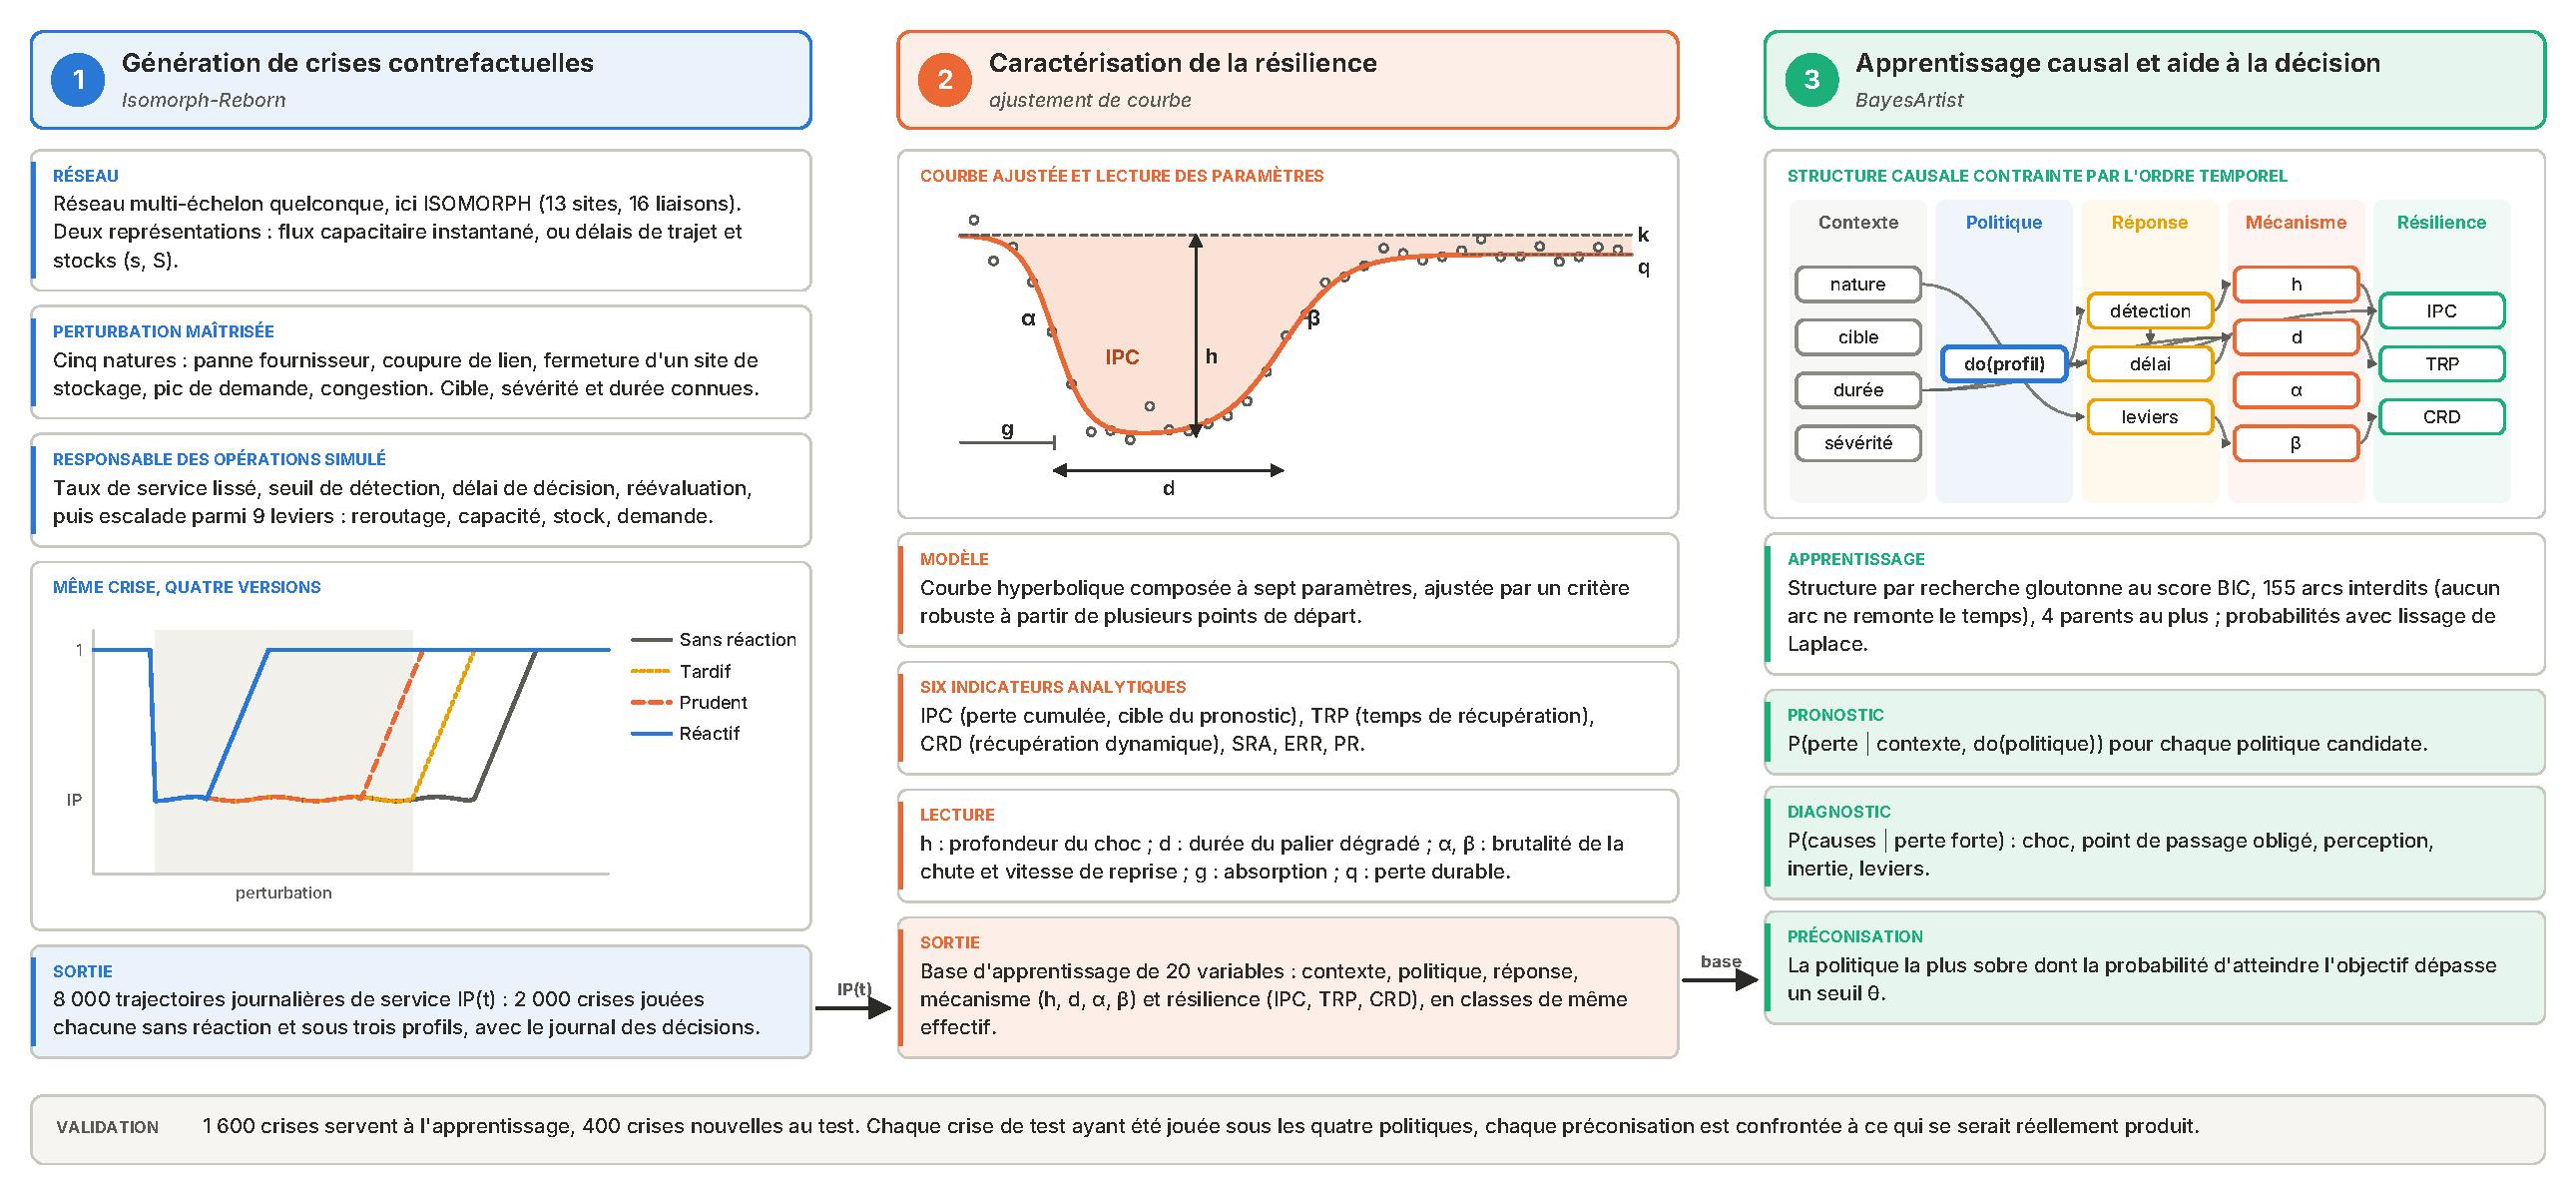
\includegraphics[width=\textwidth]{figures/Fig1_demarche.pdf}
\captionof{figure}{Démarche détaillée en trois blocs : entrées, traitements et sorties de chaque bloc.}\label{fig:demarche-detail}
\end{minipage}\end{center}

\section{Compléments sur le générateur de scénarios (Simuler)}
\label{sec:S2}

\subsection{Réseaux de référence}
\label{sec:S2.1}

Deux réseaux servent de référence (tableau~\ref{tab:reseaux}). Le réseau paramétrique comporte trois échelons : trois usines, neuf entrepôts et un client final. Chaque entrepôt est approvisionné par une usine principale, par une usine de secours via un lien de moindre capacité et, pour un entrepôt sur trois, par une troisième usine. La redondance est donc partielle par construction, et la perte de la voie principale d'un entrepôt ne peut être que partiellement compensée par ses voies de repli, comme dans la plupart des réseaux réels où la double source reste coûteuse.

Le réseau ISOMORPH reprend la topologie d'origine (Fig.~\ref{fig:d2}) : treize villes reliées par seize liaisons, avec un hub et cinq échelons intermédiaires entre les sources et le client. Le fichier d'origine ne fixant pas toutes les grandeurs nécessaires, trois hypothèses complètent sa description. La capacité de chaque liaison est tirée à plus ou moins 10~\% autour de sa valeur d'origine. La capacité de production de chaque source est fixée à 0,8 fois la capacité cumulée de ses liaisons sortantes ; à 1,0, la production ne pourrait jamais constituer un goulot et le report de charge vers les sites de production sains serait sans effet. Le dernier kilomètre est enfin supposé illimité ; les deux derniers sites de stockage avant le client n'ont alors ni capacité propre ni liaison sortante limitée, et échappent aux leviers d'expédition.

\begin{center}
% Figure : réseau ISOMORPH d'origine par échelons (données : reseau_isomorph-originel.json)
\begin{tikzpicture}[x=2.25cm,y=1cm,
  site/.style={draw=black!60, rounded corners=2pt, fill=white, font=\scriptsize, minimum width=1.75cm, minimum height=0.6cm, align=center, inner sep=1.5pt},
  usine/.style={site, fill=black!6, rounded corners=0pt},
  oblige/.style={site, draw=polreac, very thick, fill=polreac!12},
  client/.style={site, rounded corners=7pt, fill=black!12},
  arc/.style={-{Stealth[length=1.6mm]}, black!45, thin},
  arcob/.style={-{Stealth[length=2mm]}, polreac, very thick},
  delai/.style={font=\tiny, fill=white, inner sep=0.6pt, text=black!70}]
  % échelons
  \node[usine] (SF) at (0, 1.6) {San Francisco};
  \node[usine] (SL) at (0, 0)   {St. Louis};
  \node[usine] (OR) at (0,-1.6) {Orlando};
  \node[oblige] (NA) at (1, 0) {Nashville\\(hub)};
  \node[oblige] (AT) at (2, 0) {Atlanta};
  \node[site] (CH) at (3, 1.6) {Chicago};
  \node[site] (CT) at (3, 0)   {Charlotte};
  \node[site] (ME) at (3,-1.6) {Memphis};
  \node[site] (CO) at (4, 1.2) {Columbus};
  \node[site] (RI) at (4,-0.4) {Richmond};
  \node[site] (PH) at (5, 1.0) {Philadelphia};
  \node[site] (BA) at (5,-1.2) {Baltimore};
  \node[client] (NY) at (6, 0) {New York\\(client)};
  % liaisons et délais de trajet (jours)
  \draw[arc] (SF) -- node[delai]{4} (NA);
  \draw[arc] (SL) -- node[delai]{2} (NA);
  \draw[arc] (OR) -- node[delai]{2} (NA);
  \draw[arcob] (NA) -- node[delai]{1} (AT);
  \draw[arc] (AT) -- node[delai]{8} (CH);
  \draw[arc] (AT) -- node[delai]{7} (CT);
  \draw[arc] (AT) -- node[delai]{7} (ME);
  \draw[arc] (CH) -- node[delai]{2} (CO);
  \draw[arc] (CT) -- node[delai]{2} (RI);
  \draw[arc] (CO) -- node[delai,pos=0.4]{2} (PH);
  \draw[arc] (CO) -- node[delai,pos=0.25]{3} (BA);
  \draw[arc] (RI) -- node[delai,pos=0.25]{1} (PH);
  \draw[arc] (RI) -- node[delai,pos=0.4]{3} (BA);
  \draw[arc] (ME) -- node[delai]{2} (BA);
  \draw[arc] (PH) -- node[delai]{1} (NY);
  \draw[arc] (BA) -- node[delai]{2} (NY);
  % échelons
  \foreach \x/\t in {0/Sources, 1/Hub, 2/{Échelon 2}, 3/{Échelon 3}, 4/{Échelon 4}, 5/{Échelon 5}, 6/Client}
    \node[font=\scriptsize\itshape, text=black!55] at (\x, 2.45) {\t};
  % légende
  \begin{scope}[shift={(0,-2.75)}]
    \draw[arcob] (0.9,0) -- (1.35,0);
    \node[font=\scriptsize, anchor=west] at (1.4,0) {point de passage obligé : sa perte déconnecte toutes les sources du client};
    \node[font=\scriptsize, anchor=west] at (1.4,-0.5) {chiffre sur une liaison : délai de trajet en jours ; dernier kilomètre illimité};
  \end{scope}
\end{tikzpicture}

\captionof{figure}{Réseau ISOMORPH d'origine représenté par échelons, des trois sources au client.}\label{fig:d2}
\end{center}

\begin{table}[htbp]
\caption{Caractéristiques des deux réseaux de référence (valeurs nominales).}
\label{tab:reseaux}
\footnotesize
\begin{tabularx}{\textwidth}{@{}P{4.2cm}LL@{}}
\toprule
\textbf{Élément} & \textbf{Réseau paramétrique} & \textbf{Réseau ISOMORPH} \\
\midrule
Sites et échelons & 3 usines, 9 entrepôts, 1 client & 13 villes, 16 liaisons, 1 hub, 5 échelons intermédiaires \\
Capacité de production d'une source (unités par jour) & 200 à 320 & 0,8 fois la capacité de ses liaisons sortantes \\
Capacité des liaisons (unités par jour) & Voie principale 60 à 110 ; voie de secours 15 à 35 ; troisième voie 10 à 20 & Valeur d'origine $\pm$ 10~\% ; dernier kilomètre illimité \\
Capacité d'expédition d'un site de stockage (unités par jour) & 50 à 100 & Portée par les liaisons sortantes \\
Délai de trajet, représentation temporelle (jours) & 0 par défaut, réglable & 1 à 8 (valeurs d'origine) \\
Délai de production, représentation temporelle (jours) & 0 par défaut, réglable & 0 par défaut, réglable \\
Part des articles critiques dans la demande & 15~\% à 45~\% & 15~\% à 45~\% \\
Fluctuation journalière de la demande & $\pm$ 3~\% à $\pm$ 8~\% & $\pm$ 3~\% à $\pm$ 8~\% \\
\bottomrule
\end{tabularx}
\end{table}

Dans la représentation par flux, le volume livrable $F(t)$ d'un jour est la quantité maximale que le réseau peut acheminer des sources au client compte tenu de toutes ses capacités, dégradées ou renforcées ce jour-là. Cette formulation fait apparaître les goulots d'étranglement, et c'est souvent la capacité d'expédition des sites de stockage, et non la production, qui limite le service. Dans la représentation temporelle, $F(t)$ désigne le volume que la circulation de la matière et les stocks permettent effectivement de livrer ce jour-là.

\subsection{Représentation temporelle : délais et politique de stock}
\label{sec:S2.2}

La représentation par flux suppose que la matière circule instantanément et qu'aucun stock ne s'interpose entre les capacités et le client. La représentation temporelle lève ces deux hypothèses. Chaque liaison a un délai de trajet et chaque site de production un délai de production, exprimés en jours entiers. Les commandes remontent instantanément vers l'amont, mais la matière met le temps de ces délais à descendre vers le client. Chaque site de stockage gère son stock selon une politique (s, S) \citep{scarf1960} : lorsque sa position de stock, stock disponible plus matière en route, passe sous le point de commande s, il commande la quantité qui la ramène au niveau S.

Les niveaux $s_{i}$ et $S_{i}$ d'un site de stockage i sont exprimés en jours de couverture de son propre débit nominal, auxquels s'ajoute le stock nécessairement en transit vers lui :

\begin{equation}
s_i = c_s\,\Phi_i + \sum_{a \in A_i} (L_a + P_a)\, f_a, \qquad S_i = c_S\,\Phi_i + \sum_{a \in A_i} (L_a + P_a)\, f_a
\label{eq:S1}
\end{equation}

$\Phi_{i}$ désigne le débit nominal du site i, somme des débits nominaux de ses liaisons d'approvisionnement pour la demande de référence (section~3.2 du manuscrit), $c_{s}$ et $c_{S}$ les couvertures en jours, 3 et 10 jours par défaut, $A_{i}$ l'ensemble des liaisons qui approvisionnent le site i, $L_{a}$ le délai de trajet de la liaison a, $P_{a}$ le délai de production de son site d'origine et $f_{a}$ son débit nominal. Le second terme applique la loi de Little \citep{little1961} liaison par liaison. Il dimensionne la matière en route pour qu'en régime établi le stock disponible corresponde à la couverture choisie, quelle que soit l'hétérogénéité des délais d'approvisionnement. Rapporter la couverture au débit propre de chaque site, plutôt qu'à une part égale de la demande, est indispensable sur un réseau en série, sinon un hub par lequel transite tout le flux recevrait la même couverture qu'un entrepôt secondaire, et le réseau cesserait de livrer même sans perturbation. Lorsque la description du réseau fixe les niveaux d'un site, ceux-ci sont conservés.

Trois règles complètent la représentation. Chaque jour, un site de stockage sert d'abord les besoins du jour, puis le recomplètement des sites en aval, et la répartition privilégie la liaison principale avant les liaisons de secours. Les articles critiques et ordinaires sont agrégés dans les stocks, la priorité aux articles critiques ne s'appliquant qu'au service du client. Les liaisons vers le client sont enfin servies le jour même. Avec un délai sur ces liaisons, le client recevrait aujourd'hui ce qu'il a commandé la veille, et l'indicateur baisserait à chaque hausse de la demande d'un jour à l'autre, même sans perturbation ; il mesurerait alors le bruit de la demande et non la disponibilité du réseau.

Avant toute observation, le réseau est simulé sans perturbation pendant une pré-chauffe de 60 jours, qui amène les stocks et la matière en route à leur régime établi. Cette pré-chauffe est commune aux quatre versions d'une même crise.

Les deux représentations sont emboîtées. À délais nuls, la représentation temporelle reproduit presque exactement la représentation par flux, avec un écart moyen du taux de service compris entre 0,00025 et 0,002 selon les cas testés. Avec des délais, en revanche, les stocks modifient profondément la réponse du réseau aux chocs, dans une mesure qui dépend de la couverture et de la nature du choc ; la section~S5.4 en analyse la sensibilité.

\subsection{Perturbations et calibration de la demande de référence}
\label{sec:S2.3}

La coupure de lien illustre un phénomène souvent sous-estimé, car la perte d'une voie principale ne se limite pas au volume qu'elle portait. Le site de stockage privé de son approvisionnement habituel doit se réorganiser dans l'urgence, ce qui dégrade sa propre capacité d'expédition, et ses voies de secours, sursollicitées, perdent elles aussi de leur efficacité. La perturbation se propage ainsi au-delà de sa cible. Coupures et fermetures sont traitées comme des ruptures quasi totales, d'où une sévérité plus élevée ; la durée de toute perturbation varie de 3 à 15 jours. Dans la représentation temporelle, ces réductions de capacité s'appliquent de la même manière, mais leur effet sur le client est amorti par les stocks et décalé par la matière déjà en route.

L'effet d'une perturbation dépend autant de sa sévérité que de la tension dans laquelle opère le réseau, et un réseau qui dispose de marges absorbe un choc qui ferait rompre un réseau saturé. Pour contrôler ce facteur, la demande de référence de chaque scénario est fixée en fonction du volume encore livrable pendant l'incident, à l'aide d'un taux de tension $u$ tiré entre 0,85 et 1,15 :

\begin{equation}
D_{max} = \min\left(\frac{u \cdot F_{inc}}{m_{inc}},\ \frac{0{,}995 \cdot F_{nom}}{1 + \varepsilon}\right)
\label{eq:S2}
\end{equation}

$F_{\mathrm{inc}}$ et $F_{\mathrm{nom}}$ désignent le volume livrable pendant l'incident et en régime normal, $m_{\mathrm{inc}}$ la multiplication de la demande pendant l'incident (1 + 2s pour un pic de demande, 1 sinon) et $\varepsilon$ l'amplitude de la fluctuation journalière. $D_{\max}$ est la demande la plus élevée que le réseau sert à la fois pendant l'incident, à la tension $u$ près, et sans dégradation en régime normal. Les volumes $F_{\mathrm{inc}}$ et $F_{\mathrm{nom}}$ sont obtenus par un calcul de flot maximal (algorithme d'Edmonds-Karp). Le facteur $0{,}995$ laisse une marge de $0{,}5\,\%$ sous la capacité nominale. Cette marge ne se déduit d'aucune théorie ; c'est un paramètre du simulateur fixé par essais. D'abord prise à $0{,}97$, elle a été resserrée à $0{,}995$ parce qu'une marge plus large écrasait l'effet d'une coupure de lien dans un réseau redondant. Une tension inférieure à 1 réduit seulement la marge du réseau ; une tension supérieure à 1 crée une pénurie franche. Le second terme garantit, dans la représentation par flux, qu'aucune dégradation n'apparaît avant la perturbation, pendant une période initiale de 10 jours, de sorte que tout creux observé est imputable à la crise. Dans cette représentation, la demande de référence $D_{0}$ est égale à $D_{\max}$, arrondie à l'entier.

Dans la représentation temporelle, $F_{\mathrm{inc}}$ et $F_{\mathrm{nom}}$ sont mesurés par le moteur de simulation lui-même, en flux tendu : ce sont les volumes que la circulation de la matière permet effectivement d'écouler, qui ne dépassent jamais le flot maximal. Le second terme ne suffit plus alors à garantir l'absence de dégradation, car les recomplètements par à-coups et les délais peuvent laisser une demande non servie un jour donné, même sans perturbation. La demande de référence est donc vérifiée par simulation. Chaque scénario est simulé sans perturbation, pré-chauffe comprise, avec sa propre série de fluctuations, et $D_{0}$ est la plus grande demande entière au plus égale à $D_{\max}$ qui est servie intégralement chaque jour :

\begin{equation}
D_0 = \max\left\{\, d \in \mathbb{N}^*,\ d \le D_{max} \;:\; \mathrm{IP}_d(t) = 1 \ \text{pour tout jour } t \text{ simulé sans perturbation} \right\}
\label{eq:S3}
\end{equation}

$\mathrm{IP}_{d}(t)$ désigne le taux de service obtenu sous une demande de référence $d$, les niveaux s et S étant recalculés par l'équation~\eqref{eq:S1} pour chaque demande essayée. La recherche procède par dichotomie sur les entiers et ne fait qu'abaisser $D_{\max}$ ; la valeur retenue est toujours vérifiée par simulation. Lorsque même une demande d'une unité n'est pas servie intégralement, la couverture de stock est trop faible au regard des fluctuations et des délais. Le scénario n'admet aucun régime nominal sans dégradation, et le plan d'expériences est refusé plutôt que poursuivi avec une demande arbitraire. Cette condition de faisabilité relie directement la couverture de stock, les délais d'approvisionnement et la variabilité de la demande.

\subsection{Leviers de remédiation}
\label{sec:S2.4}

Les neuf leviers du gestionnaire simulé (section 3.2 du manuscrit) sont détaillés au tableau~\ref{tab:d4}.

\begin{table}[htbp]
\caption{Leviers de remédiation.}
\label{tab:d4}
\footnotesize
\begin{tabularx}{\textwidth}{@{}P{1.0cm}P{1.5cm}LLL@{}}
\toprule
\textbf{Levier} & \textbf{Famille} & \textbf{Action} & \textbf{Effet nominal} & \textbf{Perturbations concernées} \\
\midrule
D1 & Reroutage & Report de charge vers les sites de production sains & + 20 \% de capacité & Panne, coupure, congestion \\
D2 & Reroutage & Report vers les sites de stockage voisins & + 25 \% d'expédition & Coupure, fermeture, congestion \\
D3 & Capacité & Heures supplémentaires au site de production touché & 50 \% de la perte récupérée & Panne \\
D4 & Capacité & Transporteur d'appoint sur la liaison ou le site touché & 50 \% de la perte récupérée & Coupure, fermeture \\
D5 & Capacité & Entrepôt tampon & + 15 \% d'expédition sur tout le réseau & Toutes \\
D6 & Stock & Déstockage de sécurité & Flux : 30 \% de la demande, épuisé en 10 jours. Temporel : réserve séparée libérée une fois, réservée à la demande non servie & Toutes \\
D7 & Stock & Pré-positionnement près du client & Flux : 20 \% de toute perte compensée. Temporel : s et S relevés de 50 \%, commande immédiate & Panne, coupure, congestion \\
D8 & Demande & Priorisation des articles critiques & $-$ 25 \% de demande ordinaire servie & Toutes \\
D9 & Demande & Report de la demande non critique & 30 \% de la demande ordinaire différée & Toutes \\
\bottomrule
\end{tabularx}
\end{table}

Les leviers n'agissent pas tous de la même manière. Le reroutage et la capacité additionnelle restaurent ou contournent une capacité perdue. Le déstockage apporte un soulagement temporaire, qui peut produire un second creux lorsque le stock est épuisé avant la fin de la crise. Les leviers de demande, enfin, améliorent le taux de service mesuré en renonçant à une partie de la demande ordinaire ; ils traduisent un arbitrage de service plutôt qu'une restauration de la capacité, distinction qui devra guider l'interprétation des préconisations.

Dans la représentation temporelle, les deux leviers de stock changent de mécanisme. Le pré-positionnement (D7) relève temporairement les niveaux s et S des sites de stockage et déclenche une commande immédiate. Le déstockage (D6) libère une réserve de sécurité tenue à l'écart du stock ordinaire. Cette réserve est invisible de la politique de commande et ne sert que la demande que le stock ordinaire n'a pu satisfaire.

Ce mécanisme répond à un effet constaté en cours de développement. Injectée directement dans le stock ordinaire, la même quantité faisait passer certains sites au-dessus de leur point de commande. Ils sautaient alors un recomplètement, le besoin manquant remontait jusqu'aux sources, qui restaient à l'arrêt un jour de panne, et la capacité de production ainsi perdue ne se rattrapait pas. Sur un cas mesuré, le levier réduisait le volume livré au lieu de l'accroître. Une intervention d'urgence sur les stocks peut donc perturber le signal de réapprovisionnement qu'elle devait soulager. La réserve séparée garantit que le déstockage ne réduit jamais le volume livré. Les deux leviers de stock excluent enfin les sites de stockage sans capacité propre et à liaisons sortantes illimitées, sur lesquels ils n'ont pas de prise.

\subsection{Plan d'expériences, niveau de tension et contenu des observations}
\label{sec:S2.5}

Les caractéristiques du réseau, la nature, la cible, la sévérité et la durée de la perturbation, ainsi que la tension du réseau, sont tirées indépendamment pour chaque scénario, selon une loi uniforme. Les grandeurs continues sont tirées uniformément sur les plages décrites ci-dessus : capacités des sites et des liaisons, part des articles critiques, amplitude de la fluctuation de la demande, sévérité, durée (arrondie au jour) et taux de tension. La nature de la perturbation est tirée uniformément parmi les cinq natures, et sa cible parmi les sites ou liaisons admissibles ; une coupure de lien vise toutefois la liaison principale d'un site avec une probabilité de 0,85, car couper une voie de secours déjà marginale n'aurait presque aucun effet. La fluctuation journalière de la demande est elle aussi tirée uniformément, chaque jour, entre $-\varepsilon$ et $+\varepsilon$. Faute de données de terrain sur la fréquence des crises, la loi uniforme donne le même poids à toutes les valeurs plausibles et couvre l'espace des scénarios sans privilégier un régime ; les proportions observées dans la base décrivent donc cet espace, et non la fréquence réelle des crises. Tous les tirages proviennent d'un générateur pseudo-aléatoire initialisé par une graine. Le réseau de référence, la représentation et, dans la représentation temporelle, les délais par défaut et la couverture de stock sont en revanche fixés pour un lot de scénarios, et comparer plusieurs réseaux ou plusieurs couvertures suppose de générer plusieurs lots. Chaque crise est suivie sur 60 jours après son déclenchement. La génération est reproductible à l'identique, ce qui permet de régénérer une base ou de l'étendre.

Toutes les valeurs posées par hypothèse faute de données de terrain peuvent être modifiées : capacités, effets des leviers, caractéristiques des profils, hypothèses qui complètent le réseau ISOMORPH et paramètres de la représentation temporelle. Pour explorer des contextes contrastés, un niveau de tension global, de 0 à 100, déplace simultanément quatre groupes d'hypothèses : l'intensité et la durée des chocs, la tension du réseau, l'efficacité des leviers et la réactivité des gestionnaires. Le niveau 50 correspond aux valeurs nominales présentées ici. Le niveau 0 décrit un réseau surcapacitaire soumis à des chocs brefs et géré par des décideurs très réactifs ; le niveau 100 décrit des chocs de 12 à 32 jours sur un réseau saturé, avec des leviers peu efficaces et des délais de décision allant jusqu'à 12 jours. Lorsque le réseau est imposé, ce niveau continue de piloter la sévérité et la durée des chocs, la tension entre demande et capacité, l'efficacité des leviers et la réactivité des gestionnaires, mais ne modifie pas les capacités du réseau, qui viennent de sa description. Il ne touche pas non plus aux délais ni à la couverture de stock, qui relèvent de la représentation du réseau et non de l'intensité de la crise.

Chaque version d'une crise constitue une observation complète, qui réunit le contexte du réseau (identité et taille du réseau, demande de référence, part des articles critiques), la perturbation subie, le journal des décisions (date de détection, leviers mobilisés et dates d'engagement) et la trajectoire journalière du taux de service. Les niveaux de stock et la matière en route ne sont pas enregistrés, car la base décrit une crise par ses causes, ses décisions et le service rendu, et non par l'état interne du réseau. Des grandeurs descriptives simples, taux de service minimal, service cumulé perdu et délai de retour à la normale, servent au contrôle de la base.

\section{Compléments sur la courbe de résilience et les indicateurs (Mesurer)}
\label{sec:S3}

\subsection{Paramètres et estimation}
\label{sec:S3.1}

Le tableau~\ref{tab:d6} donne la lecture opérationnelle des sept paramètres de la courbe (équation~(2) du manuscrit).

\begin{table}[htbp]
\caption{Paramètres de la courbe de résilience.}
\label{tab:d6}
\footnotesize
\begin{tabularx}{\textwidth}{@{}P{1.4cm}P{3.4cm}L@{}}
\toprule
\textbf{Paramètre} & \textbf{Signification} & \textbf{Lecture pour la chaîne logistique} \\
\midrule
$k$ & Niveau avant la perturbation & Service nominal du réseau \\
$h$ & Profondeur de la chute & Ampleur de la perte de service au plus fort de la crise \\
$q$ & Écart entre niveau final et niveau initial & Perte durable ($q$ $<$ 0) ou sur-récupération ($q$ $>$ 0) \\
$g$ & Décalage de la chute & Temps pendant lequel le réseau absorbe le choc avant de se dégrader, par ses marges de capacité et, en représentation temporelle, par ses stocks et la matière en route \\
$d$ & Durée entre chute et reprise & Durée du palier dégradé, liée à la persistance du choc, au délai de réaction et, en représentation temporelle, au temps de reconstitution des stocks après le retour des capacités \\
$\alpha$ & Raideur de la chute & Brutalité de la dégradation \\
$\beta$ & Raideur de la reprise & Rapidité du rétablissement \\
\bottomrule
\end{tabularx}
\end{table}

Quelques contraintes garantissent une forme interprétable : le palier dégradé reste positif, le niveau final reste au-dessus du palier, et les raideurs ainsi que la durée du palier ne peuvent descendre sous des valeurs minimales qui produiraient des formes sans signification.

Chaque trajectoire est recalée sur le déclenchement de la perturbation, de sorte que la période précédant la crise fournit directement le niveau nominal. Les sept paramètres sont estimés en minimisant un critère robuste qui pénalise les grands écarts moins fortement que les moindres carrés :

\begin{equation}
L(\theta) = \sum_{i} 2\left(\sqrt{1 + \frac{r_i^2}{f^2}} - 1\right), \qquad r_i = p(x_i;\theta) - \mathrm{IP}(x_i), \qquad f = 0{,}05
\label{eq:S4}
\end{equation}

Ce critère, ses raisons et un exemple d'ajustement sont présentés en section 3.3 du manuscrit (figure~3).

\subsection{Définition et formules des six indicateurs}
\label{sec:S3.2}

Le tableau~\ref{tab:d7} présente les six indicateurs, la dimension de la résilience que chacun décrit et leur sens favorable.

\begin{table}[htbp]
\caption{Les six indicateurs de résilience.}
\label{tab:d7}
\footnotesize
\begin{tabularx}{\textwidth}{@{}P{3.6cm}P{2.3cm}LP{2.1cm}@{}}
\toprule
\textbf{Indicateur} & \textbf{Dimension} & \textbf{Interprétation} & \textbf{Sens favorable} \\
\midrule
IPC, indice de perte cumulée & Perte & Service cumulé perdu pendant la crise & Faible \\
CRD, coefficient de récupération dynamique & Vitesse & Rapidité de la reprise rapportée à la chute et à la durée du palier & Élevé \\
TRP, temps de récupération pondéré & Durée & Temps nécessaire pour que la reprise atteigne 95~\% de son amplitude & Faible \\
SRA, score de robustesse adaptative & Adaptation & Capacité à remonter, pénalisée par un écart durable au niveau initial & Élevé \\
ERR, efficacité de résilience relative & Performance conservée & Part du service nominal maintenue sur l'épisode & Élevé \\
PR, potentiel de récupération & Rétablissement & Niveau final rapporté à la mi-profondeur de la chute & À préciser \\
\bottomrule
\end{tabularx}
\end{table}

Six indicateurs sont calculés analytiquement à partir des paramètres ajustés. Ils héritent ainsi du lissage opéré par l'ajustement et décrivent chacun une facette de la résilience : perte subie, vitesse et durée de la reprise, capacité d'adaptation, performance conservée et potentiel de rétablissement.

\begin{align}
\mathrm{IPC} &= \frac{h}{\alpha}\ln 2 + \frac{h\,d}{2} - \frac{h + q}{\beta}\ln 2 \label{eq:S5} \\
\mathrm{CRD} &= \frac{\beta}{\alpha}\cdot\frac{h + q}{h}\cdot\frac{1}{d}\cdot\sqrt{\alpha\beta} \label{eq:S6} \\
\mathrm{TRP} &= d + \frac{2{,}95}{\beta} \label{eq:S7} \\
\mathrm{SRA} &= \frac{\beta\,(h + q)}{\alpha\,h\,d}\, e^{-|q|/h}\,\big(1 + \tanh(\beta - \alpha)\big) \label{eq:S8} \\
\mathrm{ERR} &= 1 + \frac{q}{2k} - \frac{h\,|\mathrm{IPC}|}{T\,k}, \quad T = g + d + \frac{4}{\beta} \label{eq:S9} \\
\mathrm{PR} &= \frac{k + q}{k - h/2} \label{eq:S10}
\end{align}

L'horizon $T$ de l'équation~\eqref{eq:S9} couvre la chute et une reprise complète à environ 98 \%, conformément à la définition proposée par \citet{rahiel2026in4pl} ; il s'adapte ainsi à la durée propre de chaque crise au lieu d'imposer une fenêtre fixe.

\subsection{Qualité d'ajustement, cas limites et domaine de la résilience}
\label{sec:S3.3}

La qualité de chaque ajustement est appréciée par le coefficient de détermination et l'erreur quadratique moyenne, calculés sur la trajectoire brute, ainsi que par un coefficient de détermination calculé sur la trajectoire lissée sur cinq jours. L'écart entre les deux coefficients distingue un défaut de forme de la courbe d'une simple fluctuation journalière de la demande. Les crises dont l'ajustement est insuffisant, ou dont la chute est trop faible pour être caractérisée, peuvent être écartées de la base.

Les crises absorbées sans dégradation notable, lorsque le réseau dispose d'assez de marge ou, en représentation temporelle, d'assez de stock, posent une première difficulté : la profondeur $h$ tend vers zéro et les indicateurs rapportés à $h$, CRD et SRA, deviennent instables. La couverture de stock permet de déplacer de manière contrôlée le seuil à partir duquel une crise est ainsi absorbée. Les trajectoires à plusieurs creux se rencontrent typiquement lorsqu'un stock mobilisé s'épuise avant la fin de la crise, ou lorsque le retour des capacités provoque un rétablissement brutal : la courbe n'en restitue qu'une enveloppe. Enfin, PR augmente avec la profondeur de la chute à niveau final donné ; son sens d'interprétation doit être arrêté avant de l'utiliser comme objectif de pilotage.

Ces cas limites tiennent à la définition même de la résilience. Trois propriétés voisines se distinguent par la forme de la trajectoire du taux de service. La robustesse est la capacité à absorber un choc sans dégradation notable : le taux de service reste au niveau nominal et il n'y a rien à rétablir. La stabilité est la capacité à rester au voisinage de ce niveau malgré des variations rapides et de faible amplitude, comme les fluctuations journalières de la demande, qui relèvent de la régulation courante. La résilience suppose au contraire une chute effective, suivie d'un rétablissement : elle se mesure à la perte subie et à la manière dont le taux de service revient à un niveau acceptable. Son domaine est donc borné des deux côtés. Sans chute, la question de la résilience ne se pose pas ; lorsque la chute est telle que le réseau cesse durablement de servir et ne se rétablit pas sur la période observée, la crise relève de la défaillance, qui appelle une reconfiguration plutôt qu'un rétablissement. La courbe hyperbolique composée \citep{rahiel2026in4pl} est construite pour ce domaine, qui va d'une chute à une reprise. L'instabilité de CRD et SRA lorsque $h$ tend vers zéro signale ainsi une crise absorbée, c'est-à-dire un cas de robustesse, et non une limite du modèle.

\subsection{Signatures des dysfonctionnements sur la courbe}
\label{sec:S3.4}

Les paramètres de la courbe relient la trajectoire observée aux mécanismes décrits en section 3 du manuscrit. Le tableau~\ref{tab:S3} résume les signatures attendues ; il constitue un ensemble d'hypothèses que l'analyse des résultats et l'apprentissage causal permettent de confirmer ou de nuancer.

\begin{table}[htbp]
\caption{Signatures des dysfonctionnements sur la courbe de résilience.}
\label{tab:S3}
\footnotesize
\begin{tabularx}{\textwidth}{@{}LLL@{}}
\toprule
\textbf{Phénomène} & \textbf{Signature attendue sur la courbe} & \textbf{Origine probable} \\
\midrule
Absorption du choc & $h$ faible, $g$ élevé & Marges de capacité, voies de secours suffisantes \\
Absorption par les stocks & $h$ faible ou nul, $g$ élevé & Couverture de stock élevée au regard de la durée du choc \\
Rupture brutale & $h$ élevé, $\alpha$ élevé & Coupure ou fermeture sévère, réseau sous tension \\
Rupture différée & $g$ élevé, puis $h$ élevé & Stocks épuisés en cours de crise, matière en route insuffisante \\
Dégradation progressive & $\alpha$ faible & Congestion diffuse, pic de demande modéré \\
Crise prolongée & $d$ élevé & Perturbation longue, détection tardive, inertie décisionnelle \\
Reprise retardée & $d$ supérieur à la durée du choc & Reconstitution des stocks et de la matière en route après le retour des capacités \\
Reprise rapide & $\beta$ élevé, TRP faible & Levier efficace engagé tôt \\
Perte durable & $q$ $<$ 0 & Capacité non restaurée à la fin de la période, stock épuisé \\
Sur-récupération & $q$ $>$ 0 & Leviers maintenus après la fin de la perturbation \\
\bottomrule
\end{tabularx}
\end{table}

\section{Compléments sur l'apprentissage du réseau bayésien (Apprendre)}
\label{sec:S4}

\subsection{Construction de la base d'apprentissage}
\label{sec:S4.1}

Chaque version d'une crise, c'est-à-dire une crise jouée sous un comportement de gestion donné, fournit une observation ; la base principale en compte 8 000. Les variables sont organisées selon les causes qu'un diagnostic doit pouvoir distinguer : l'exposition du réseau, la perturbation, la politique de gestion et la réponse effective du gestionnaire, complétées par le mécanisme de la chute et par la résilience obtenue (tableau~5 du manuscrit).

La demande de référence n'est pas une variable de contexte : calibrée sur le volume livrable pendant l'incident, elle dépend de la perturbation elle-même. Elle est remplacée par la position de la cible dans la topologie : un site ou une liaison constitue un point de passage obligé si sa suppression déconnecte toutes les sources du client. Sur le réseau ISOMORPH, le hub de Nashville, l'entrepôt d'Atlanta et la liaison qui les relie sont dans ce cas ; la congestion et le pic de demande touchent le réseau entier. Cette variable ne dépend que de la structure du réseau et se transpose à tout réseau étudié. La politique est représentée par le profil seul : ses composantes (seuil, délai, rythme, ordre des leviers) lui sont parfaitement redondantes dans une base où elles sont fixées par profil. Une réponse absente, lorsque le taux de service n'est jamais passé sous le seuil critique, est codée par un état explicite « sans objet ».

Les paramètres de la courbe sont conservés comme variables intermédiaires : ils décrivent le mécanisme par lequel une cause produit son effet (tableau~\ref{tab:S3}). Trois sont écartés faute de variation dans la base : $k$, proche de 1 par construction, $q$, proche de 0 parce que les crises se résorbent avant la fin de la période observée, et $g$, presque toujours nul. Parmi les indicateurs, IPC, fidèle au service perdu et sans ambiguïté de sens, sert de cible au pronostic ; TRP et CRD le complètent. SRA, redondant avec les paramètres, ERR, trop peu dispersé, et PR, dont le sens favorable dépend de la profondeur de la chute, sont écartés.

Toutes les versions sont conservées, y compris celles dont l'ajustement est imparfait : écarter les crises mal ajustées éliminerait surtout les crises courtes, donc une partie des réussites du profil réactif. Les variables continues sont discrétisées en trois classes de même effectif, dont les seuils sont calculés sur l'échantillon d'apprentissage puis figés pour les crises nouvelles.

\subsection{Apprentissage sous contraintes}
\label{sec:S4.2}

L'apprentissage est réalisé avec l'outil BayesArtist \citep{bayesartist}. La structure est apprise par recherche locale gloutonne au critère d'information bayésien (BIC) \citep{schwarz1978}. L'ordre des paliers est imposé comme une liste d'arcs interdits, avec au plus quatre parents par variable, de sorte qu'aucune structure apprise ne peut violer la temporalité de la crise ; cette combinaison de connaissance du domaine et de données suit le principe de \citet{heckerman1995}. Les tables de probabilités sont estimées par comptage avec un lissage de Laplace, qui évite d'attribuer une probabilité nulle à une combinaison de causes absente de la base, et l'inférence est exacte, par élimination de variables ou arbre de jonction \citep{koller2009}.

La politique, intervention comparée sur des crises strictement identiques, a un effet sur la résilience identifiable sans ajustement. Les leviers effectivement mobilisés dépendent au contraire de ce que le gestionnaire a perçu : ce sont des médiateurs.

BayesArtist n'étant pas diffusé, le même apprentissage peut être conduit avec tout logiciel de réseaux bayésiens qui apprend la structure et les paramètres à partir d'un fichier CSV et accepte des arcs interdits, par exemple Hugin, GeNIe, le paquet R bnlearn ou la bibliothèque Python pgmpy ; les algorithmes de recherche différant d'un outil à l'autre, de légers écarts de structure sont possibles.

\subsection{Inférence, préconisation et protocole de validation}
\label{sec:S4.3}

En pronostic, le réseau donne la distribution de la résilience pour un contexte et une politique, par exemple la probabilité d'une perte cumulée faible face à la fermeture sévère d'un site de stockage gérée par un profil prudent. En diagnostic, il remonte d'une résilience dégradée vers les causes les plus probables : point de passage obligé touché, choc difficilement surmontable, perception tardive, inertie décisionnelle ou leviers inadaptés.

La préconisation combine les deux. Face à une nouvelle crise, décrite en tout ou partie, et à un objectif de résilience, chaque politique candidate est évaluée par la probabilité d'atteindre cet objectif, qui se lit directement dans le réseau puisque la politique est une intervention. La règle retenue privilégie la sobriété : parmi les politiques dont cette probabilité dépasse un seuil $\theta$ fixé par le décideur, est préconisée la moins interventionniste, les politiques étant ordonnées par le nombre moyen de leviers qu'elles engagent (sans réaction, tardif, prudent, réactif). Si aucune n'atteint le seuil, la politique la plus probable est préconisée. Cette règle traduit le fait que tout levier a un coût que le modèle ne valorise pas : à résilience égale, mobiliser moins de leviers est préférable.

La même question peut être posée à rebours : fixer l'objectif, par exemple une perte cumulée faible, et le contexte connu, puis lire la distribution du profil. En général, remonter d'un effet vers une décision ne livre qu'une association, car les décisions observées dépendent de la situation. Ici, le profil est une variable racine, assignée selon une loi uniforme indépendamment du contexte : sa probabilité a posteriori est donc proportionnelle à sa probabilité d'atteindre l'objectif, et l'inférence à rebours classe les politiques exactement comme le pronostic. Elle fournit en une requête par contexte une carte de préconisation, qui désigne la politique la plus efficace ; la règle de sobriété reste nécessaire pour retenir la plus économe parmi celles qui suffisent. Cette propriété ne vaut pas pour les leviers, qui dépendent de ce que le gestionnaire perçoit.

La validation exploite une propriété rare de la base : chaque crise y est observée sous les quatre politiques. Les 2 000 scénarios sont partagés aléatoirement en 1 600 scénarios d'apprentissage et 400 de test ; le découpage porte sur les scénarios, les quatre versions d'une même crise n'étant pas indépendantes. Le pronostic est jugé sur la prédiction de la classe de perte cumulée à partir des seules variables connues au moment de décider, par le taux de classement correct et le score de Brier, comparés à la classe majoritaire et à un modèle fondé sur la seule politique. Le diagnostic est jugé en confrontant, pour les crises à forte perte, la distribution a posteriori des causes à leur fréquence observée. La préconisation est jugée directement : chaque crise de test ayant été jouée sous toutes les politiques, on vérifie si la politique préconisée a effectivement atteint l'objectif, et l'on mesure la part des préconisations plus sobres que le profil réactif. Une courbe d'apprentissage, de 200 à 1 600 scénarios, indique si la taille de la base est suffisante.

\section{Résultats complémentaires}
\label{sec:S5}

\subsection{Caractéristiques de la base principale}
\label{sec:S5.1}

Cette configuration a été retenue au terme d'un essai préliminaire d'une quarantaine de configurations, sur un critère unique : le contraste entre politiques, sans lequel l'apprentissage causal n'aurait rien à identifier. La représentation par flux isole les mécanismes de capacité et rend les écarts entre politiques directement interprétables.

La base compte 2 000 scénarios, soit 8 000 versions de crise, et les cinq natures de perturbation y sont représentées de manière équilibrée (tableau~\ref{tab:d11}). La demande de référence, calibrée sur le volume encore livrable pendant l'incident (équation~\eqref{eq:S2}), est très faible lorsque la perturbation touche le hub de Nashville ou l'entrepôt d'Atlanta, par lesquels transite tout le flux : elle reflète la criticité du site touché autant que la taille du réseau.

\begin{table}[htbp]
\caption{Caractéristiques de la base principale.}
\label{tab:d11}
\footnotesize
\begin{tabularx}{\textwidth}{@{}LL@{}}
\toprule
\textbf{Caractéristique} & \textbf{Valeur} \\
\midrule
Scénarios ; versions de crise & 2 000 ; 8 000 \\
Répartition des natures & Panne fournisseur 422, fermeture d'un site de stockage 405, pic de demande 395, congestion 390, coupure de lien 388 \\
Durée de la perturbation, médiane [quartiles] & 16 jours [12 ; 20] \\
Sévérité, médiane [quartiles] & 0,91 [0,82 ; 0,95] \\
Part des articles critiques & 0,20 à 0,53 \\
Coefficient de détermination, médiane [quartiles] & 0,88 [0,79 ; 0,93] \\
Coefficient de détermination sur trajectoire lissée, médiane & 0,91 \\
Versions dont la chute est inférieure à 0,03 & 4,2 \% \\
Indicateurs non finis & 0 \\
Corrélation entre IPC et service perdu observé & 0,97 \\
\bottomrule
\end{tabularx}
\end{table}

L'ajustement est satisfaisant pour l'essentiel de la base : le coefficient de détermination médian atteint 0,88 et aucun indicateur n'est indéfini. Un quart des versions reste sous 0,8, principalement des crises courtes ou à reprise accidentée. L'indicateur de perte cumulée IPC reste néanmoins très fidèle au service effectivement perdu (corrélation de 0,97), ce qui justifie d'en faire l'indicateur principal de résilience : il dépend peu des imperfections de forme de la courbe ajustée.

\subsection{Effet des politiques selon la nature du choc et le réseau}
\label{sec:S5.2}

Les profils diffèrent aussi par les leviers engagés : le profil tardif n'engage que des leviers de demande, faute de pouvoir escalader au-delà de ses deux premiers choix pendant la crise, le profil prudent s'appuie surtout sur les stocks et la capacité additionnelle, le profil réactif sur le reroutage et la capacité. Leur efficacité dépend de la nature de la perturbation (tableau~\ref{tab:d13}).

\begin{table}[htbp]
\caption{Réduction médiane de la perte cumulée par rapport à l'absence de réaction, selon la nature de la perturbation.}
\label{tab:d13}
\footnotesize
\begin{tabularx}{\textwidth}{@{}LLLL@{}}
\toprule
\textbf{Nature} & \textbf{Réactif} & \textbf{Prudent} & \textbf{Tardif} \\
\midrule
Panne fournisseur & 84 \% & 0 \% & 0 \% \\
Coupure de lien & 73 \% & 17 \% & 0 \% \\
Fermeture d'un site de stockage & 82 \% & 10 \% & 2 \% \\
Pic de demande & 87 \% & 23 \% & 13 \% \\
Congestion & 78 \% & 41 \% & 15 \% \\
\bottomrule
\end{tabularx}
\end{table}

Le profil prudent est sans effet sur une panne fournisseur, que le déstockage ne compense pas, mais réduit de 41~\% la perte d'une congestion, choc diffus que des leviers globaux atténuent ; le profil réactif est le moins efficace face à une coupure de lien, dont les effets se propagent aux voies de secours.

Pour vérifier que ces résultats ne tiennent pas à la seule topologie d'ISOMORPH, un lot de contrôle de 500 scénarios a été généré sur le réseau paramétrique avec les mêmes réglages. Les crises y sont moins profondes (taux de service minimal médian de 0,91) et l'ajustement moins bon, mais la perte cumulée reste très fidèle au service perdu (corrélation de 0,97). Les grandes proportions sont remarquablement stables : la part du service perdu évitée atteint 67~\%, 17~\% et 13~\% pour les profils réactif, prudent et tardif, contre 73~\%, 18~\% et 14~\% sur ISOMORPH. La topologie modifie en revanche l'efficacité des leviers selon la nature du choc : sur le réseau paramétrique, dont les voies de secours sont de faible capacité, le profil réactif ne réduit plus que de 25~\% la perte d'une coupure de lien et de 53~\% celle d'une fermeture, contre 73~\% et 82~\% sur ISOMORPH. L'effet d'une politique dépend donc conjointement de la nature du choc et de la redondance du réseau.

\subsection{Pronostic, diagnostic et étude de cas}
\label{sec:S5.3}

Le pronostic, établi à partir des seules variables connues au moment de décider, classe correctement 65~\% des crises de test, contre 34~\% pour la classe majoritaire et 60~\% pour un modèle fondé sur la seule politique. Le gain apporté par le contexte est réel mais modeste. La courbe d'apprentissage est presque plate, de 62,5~\% avec 200 scénarios à 63,7~\% avec 1 600 : la taille de la base n'est pas le facteur limitant, c'est l'information disponible au moment de décider. La perte dépend notamment de la tension du réseau, que le générateur n'exporte pas.

Le diagnostic est bien calibré pour la politique et la durée. Pour les crises de test à forte perte, la probabilité a posteriori de chaque politique (sans réaction, tardif, prudent, réactif) vaut 0,42, 0,32, 0,26 et 0,01, pour des fréquences observées de 0,41, 0,33, 0,26 et 0,005 ; celle d'une perturbation longue vaut 0,41, comme sa fréquence observée. Il l'est moins pour la nature du choc et la position de la cible : les crises touchant un point de passage obligé, 6~\% de la base, sont trop rares pour que le score retienne leurs effets propres.

Deux crises de même nature illustrent l'usage du réseau. Dans la première, un site de stockage situé sur un point de passage obligé, comme l'entrepôt d'Atlanta, est fermé pour une longue durée. Le réseau (figure~\ref{fig:d7}) donne une probabilité de forte perte de 0,70 sans réaction, de 0,56 sous le profil tardif, de 0,44 sous le profil prudent et de 0,01 sous le profil réactif. Seul ce dernier atteint l'objectif avec une probabilité suffisante : la préconisation est sans ambiguïté, quel que soit le seuil retenu.

Dans la seconde, un site de stockage redondé est fermé pour une courte durée. La probabilité de forte perte tombe à 0,30 sans réaction, 0,22 sous le profil tardif et 0,20 sous le profil prudent. Avec $\theta$ = 0,8, le profil prudent atteint l'objectif avec une probabilité de 0,80 et devient la préconisation : face à un choc bref sur un site doublé, une réaction fondée sur le déstockage suffit, et mobiliser le reroutage et la capacité additionnelle n'apporterait qu'un gain marginal.

\begin{center}
% Figure : pronostic de la perte cumulée selon la politique (inférence dans BayesArtist sur le réseau appris)
% Évidences : nature = fermeture_entrepot, cible = passage_oblige, duree = fort ; valeurs lues dans BayesArtist.
\begin{tikzpicture}[x=1cm,y=1cm, font=\scriptsize]
  \node[anchor=east] at (-0.15,0.00) {Réactif};
  \fill[palmec!75] (0.000,-0.30) rectangle (10.812,0.30);
  \node at (5.406,0.00) {$0{,}90$};
  \fill[poltard!75] (10.812,-0.30) rectangle (11.904,0.30);
  \node at (11.358,0.00) {$0{,}09$};
  \fill[polprud!75] (11.904,-0.30) rectangle (11.988,0.30);
  \node[anchor=west] at (12.05,0.00) {$0{,}01$};
  \node[anchor=east] at (-0.15,-0.90) {Prudent};
  \fill[palmec!75] (0.000,-1.20) rectangle (1.272,-0.60);
  \node at (0.636,-0.90) {$0{,}11$};
  \fill[poltard!75] (1.272,-1.20) rectangle (6.672,-0.60);
  \node at (3.972,-0.90) {$0{,}45$};
  \fill[polprud!75] (6.672,-1.20) rectangle (12.000,-0.60);
  \node at (9.336,-0.90) {$0{,}44$};
  \node[anchor=east] at (-0.15,-1.80) {Tardif};
  \fill[palmec!75] (0.000,-2.10) rectangle (1.056,-1.50);
  \node at (0.528,-1.80) {$0{,}09$};
  \fill[poltard!75] (1.056,-2.10) rectangle (5.268,-1.50);
  \node at (3.162,-1.80) {$0{,}35$};
  \fill[polprud!75] (5.268,-2.10) rectangle (12.000,-1.50);
  \node at (8.634,-1.80) {$0{,}56$};
  \node[anchor=east] at (-0.15,-2.70) {Sans réaction};
  \fill[palmec!75] (0.000,-3.00) rectangle (0.816,-2.40);
  \node at (0.408,-2.70) {$0{,}07$};
  \fill[poltard!75] (0.816,-3.00) rectangle (3.600,-2.40);
  \node at (2.208,-2.70) {$0{,}23$};
  \fill[polprud!75] (3.600,-3.00) rectangle (12.000,-2.40);
  \node at (7.800,-2.70) {$0{,}70$};
  \draw[black!50] (0,-3.15) -- (12.0,-3.15);
  \foreach \p/\l in {0/0,0.2/0{,}2,0.4/0{,}4,0.6/0{,}6,0.8/0{,}8,1/1} { \draw[black!50] (\p*12.0,-3.15) -- ++(0,-0.08) node[below] {$\l$}; }
  \node[font=\small] at (6.0,-3.90) {Probabilité de chaque classe de perte cumulée IPC};
  \fill[palmec!75] (1.20,0.55) rectangle (1.55,0.8); \node[anchor=west] at (1.60,0.675) {Perte faible};
  \fill[poltard!75] (4.60,0.55) rectangle (4.95,0.8); \node[anchor=west] at (5.00,0.675) {Perte moyenne};
  \fill[polprud!75] (8.00,0.55) rectangle (8.35,0.8); \node[anchor=west] at (8.40,0.675) {Perte forte};
\end{tikzpicture}

\captionof{figure}{Pronostic de la perte cumulée selon la politique, pour la fermeture longue d'un site situé sur un point de passage obligé : distribution des trois classes d'IPC inférée par le réseau appris.}\label{fig:d7}
\end{center}

Le diagnostic éclaire le cas inverse, celui d'une crise à forte perte gérée par un profil prudent. Le réseau y associe une perturbation longue, avec une probabilité de 0,39 contre 0,33 a priori, un recours au déstockage presque certain (0,95) et une escalade jusqu'à trois leviers ou plus (0,40 contre 0,23 a priori). Il désigne ainsi une crise trop longue pour la politique choisie : le gestionnaire a escaladé, mais à partir de leviers de stock dont l'effet s'épuise, sans atteindre à temps le reroutage. Ce diagnostic oriente l'action corrective vers la politique, plus réactive ou dotée d'un autre ordre de leviers, plutôt que vers le réseau.

La figure~6 du manuscrit applique la lecture à rebours de la section~3.4 du manuscrit aux sept contextes que la topologie d'ISOMORPH rend possibles, pour l'objectif d'une perte cumulée faible. Le profil réactif est le plus probable partout, et d'autant plus que le choc dure : sa probabilité a posteriori passe de 0,51 à 0,58 pour un choc court à 0,72 à 0,79 pour un choc long. Pour un choc court, les trois autres politiques conservent chacune entre 0,12 et 0,18 : une perte faible y reste accessible sans réaction rapide, ce qui rejoint la préconisation sobre de la section~4.3 du manuscrit. La carte varie en revanche peu avec la nature du choc et la position de la cible, conformément au diagnostic : dans la structure apprise, ces variables n'agissent sur la perte qu'à travers les leviers mobilisés.

\subsection{Sensibilité à la couverture de stock}
\label{sec:S5.4}

La représentation temporelle permet d'étudier le rôle des stocks, que la base principale neutralise. Sur le réseau ISOMORPH, avec ses délais de trajet d'origine, 60 crises ont été simulées pour chaque nature de perturbation et chaque couverture, sans réaction du gestionnaire, et l'on a compté celles qui produisent une baisse de service visible (figure~\ref{fig:d8} et tableau~\ref{tab:S4}). La représentation par flux sert de référence.

\begin{center}
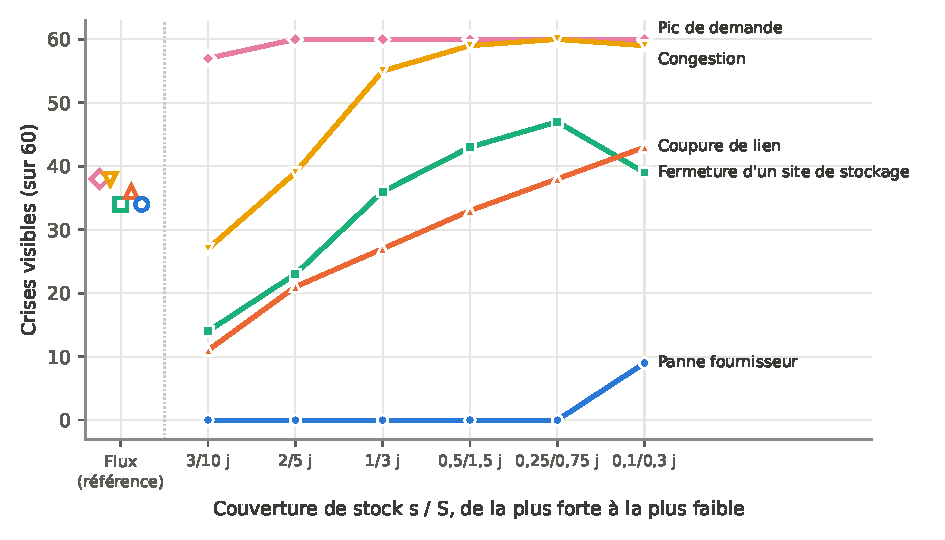
\includegraphics[width=0.75\textwidth]{figures/Fig8_couverture_stock.pdf}
\captionof{figure}{Nombre de crises visibles sur 60 selon la couverture de stock, par nature de perturbation (réseau ISOMORPH, sans réaction). Les symboles creux, à gauche, donnent la référence de la représentation par flux.}\label{fig:d8}
\end{center}

Pour les ruptures de distribution, coupure de lien, fermeture d'un site de stockage et congestion, la couverture agit comme un levier de robustesse progressif : plus elle est faible, plus les crises visibles sont nombreuses, de 11 à 43 sur 60 pour une coupure de lien et de 27 à 59 pour une congestion. La frontière entre robustesse et résilience évoquée en section~S3.3 se déplace donc de manière contrôlée avec le niveau de stock. Les pannes fournisseur sont au contraire absorbées dès que la couverture atteint un quart de jour, y compris pour des pannes de 15 à 60 jours à la couverture par défaut : la calibration de la demande borne le manque à servir pendant une panne, que quelques jours de stock suffisent à compenser. Enfin, le pic de demande est mieux absorbé sans stocks qu'avec : dans la représentation par flux, toute marge de capacité sert instantanément le surcroît de demande, alors qu'avec des délais, ce surcroît doit d'abord être prélevé sur des stocks dimensionnés sur le débit nominal, que le recomplètement ne reconstitue qu'après un délai.

La couverture de stock n'est donc pas un levier universel de résilience. Elle protège contre les pertes de capacité de distribution, est presque superflue contre une défaillance amont de faible ampleur, et ne protège pas contre un choc de demande, qui appelle des leviers de capacité ou de demande. Ces résultats, obtenus sans réaction du gestionnaire et à couverture uniforme, n'épuisent pas la question : l'interaction entre couverture et politique de gestion reste à étudier.

\begin{table}[htbp]
\caption{Crises produisant une baisse de service visible, sur 60, selon la couverture de stock (réseau ISOMORPH, sans réaction).}
\label{tab:S4}
\footnotesize
\begin{tabularx}{\textwidth}{@{}LLLLLLLL@{}}
\toprule
\textbf{Nature} & \textbf{Flux} & \textbf{3 / 10 j} & \textbf{2 / 5 j} & \textbf{1 / 3 j} & \textbf{0,5 / 1,5 j} & \textbf{0,25 / 0,75 j} & \textbf{0,1 / 0,3 j} \\
\midrule
Panne fournisseur & 34 & 0 & 0 & 0 & 0 & 0 & 9 \\
Coupure de lien & 36 & 11 & 21 & 27 & 33 & 38 & 43 \\
Fermeture d'un site de stockage & 34 & 14 & 23 & 36 & 43 & 47 & 39 \\
Pic de demande & 38 & 57 & 60 & 60 & 60 & 60 & 60 \\
Congestion & 38 & 27 & 39 & 55 & 59 & 60 & 59 \\
\bottomrule
\end{tabularx}
\end{table}

\subsection{Lecture économique détaillée et coût de la sur-réaction}
\label{sec:S5.5}

La politique réactive est à la fois la plus efficace et la plus rentable par levier : chacun de ses leviers préserve en moyenne 6 630 unités, soit environ un tiers de journée de demande. Pour une marge de 10 euros par unité, elle reste rentable tant qu'un levier coûte moins de 66 000 euros par crise. La politique prudente est au contraire économiquement dominée : elle engage plus des deux tiers des leviers de la politique réactive pour un quart de ses gains, et chaque levier qu'elle ajoute à la politique tardive ne préserve que 790 unités. Le coût d'une politique tient donc moins au nombre de leviers qu'à leur moment d'engagement : engagés tôt, ils évitent l'allongement de la crise ; engagés tard ou dans le mauvais ordre, ils arrivent quand l'essentiel de la perte est consommé. La rentabilité dépend aussi de la nature du choc : le seuil de la politique réactive atteint 13 100 unités par levier pour une panne fournisseur, mais seulement 2 300 pour une congestion, que des leviers globaux atténuent mal. Le seuil élevé de la politique tardive appelle une réserve : ses gains viennent surtout des leviers de demande, et en particulier du report de la demande non critique, qui relève le taux de service mesuré en différant des ventes plutôt qu'en les préservant. Une partie de ces gains est donc reportée sur la période suivante, et son seuil de rentabilité est probablement surestimé.

La figure~7 du manuscrit en tire la conséquence pour le choix d'une politique. Parmi les politiques fixes, la réactivité est optimale tant que le coût d'un levier reste sous le seuil de 6 630 unités de marge ; au-delà, mieux vaut ne pas réagir, et les politiques prudente et tardive ne sont jamais le meilleur choix. La courbe noire en tirets retient, pour chaque crise et chaque coût de levier, la politique au meilleur bénéfice, puis en fait la moyenne sur les 2 000 crises. Ce choix est fait a posteriori, comme si l'issue de chaque politique était connue d'avance : la courbe constitue donc une limite haute de ce qu'une préconisation adaptée à la crise peut rapporter, dont le réseau bayésien, qui ne connaît la crise que partiellement, ne capte qu'une partie. Cette limite haute conserve un bénéfice positif bien au-delà du seuil de la politique réactive, parce que pour certaines crises la politique tardive ou l'absence de réaction suffisent. Pour un levier valant 5 000 unités de marge, le choix adapté porterait le bénéfice moyen de 4 560 à 8 350 unités par crise, soit 83~\% de plus que la meilleure politique fixe ; pour un levier plus coûteux, il resterait le seul à dégager un gain. C'est la valeur économique que vise la préconisation du réseau bayésien : identifier, à partir de ce que l'on sait de la crise, celles où une politique plus sobre suffit.

Deux lots complémentaires, aux réglages du lot principal, mesurent le coût de la sur-réaction : 400 scénarios sans perturbation perceptible et 300 perturbations mineures (sévérité de 0,1 à 0,3, durée de 1 à 3 jours). Sans perturbation, aucun profil n'engage de levier : la détection, fondée sur le taux de service lissé, ne se déclenche pas sur les seules fluctuations de la demande. Face à une perturbation mineure, en revanche, le profil réactif engage au moins un levier dans 32~\% des cas, contre 4~\% pour le profil prudent et aucun pour le profil tardif, pour ne réduire les ventes perdues que de 2 335 à 2 260 unités par crise. Chaque levier y préserve environ 230 unités, près de trente fois moins que sur l'ensemble des crises de la base principale. La sensibilité du profil réactif a donc un coût réel face aux chocs mineurs, pour l'essentiel des pics de demande et des congestions : elle ne se justifie que si l'on sait distinguer un choc mineur d'une crise sévère, ce que vise le pronostic du réseau bayésien.

\section{Résultats complémentaires}
\label{sec:S6}

\subsection{Caractéristiques de la base principale}
\label{sec:S6.1}

La configuration de la base principale (réseau ISOMORPH, représentation par flux, niveau de tension 75) a été retenue après un essai préliminaire d'une quarantaine de configurations, sur un seul critère, le contraste entre politiques, sans lequel l'apprentissage causal n'aurait rien à identifier. La représentation par flux isole les mécanismes de capacité et rend les écarts entre politiques directement interprétables.

La base compte 2 000 scénarios, soit 8 000 versions de crise. Les cinq natures de perturbation y sont représentées de manière équilibrée (tableau~\ref{tab:d11}). La demande de référence, calibrée sur le volume encore livrable pendant l'incident (équation~\eqref{eq:S2}), est très faible lorsque la perturbation touche le hub de Nashville ou l'entrepôt d'Atlanta, par lesquels transite tout le flux ; elle reflète la criticité du site touché autant que la taille du réseau.

\begin{table}[htbp]
\caption{Caractéristiques de la base principale.}
\label{tab:d11}
\footnotesize
\begin{tabularx}{\textwidth}{@{}LL@{}}
\toprule
\textbf{Caractéristique} & \textbf{Valeur} \\
\midrule
Scénarios ; versions de crise & 2 000 ; 8 000 \\
Répartition des natures & Panne fournisseur 422, fermeture d'un site de stockage 405, pic de demande 395, congestion 390, coupure de lien 388 \\
Durée de la perturbation, médiane [quartiles] & 16 jours [12 ; 20] \\
Sévérité, médiane [quartiles] & 0,91 [0,82 ; 0,95] \\
Part des articles critiques & 0,20 à 0,53 \\
Coefficient de détermination, médiane [quartiles] & 0,88 [0,79 ; 0,93] \\
Coefficient de détermination sur trajectoire lissée, médiane & 0,91 \\
Versions dont la chute est inférieure à 0,03 & 4,2 \% \\
Indicateurs non finis & 0 \\
Corrélation entre IPC et service perdu observé & 0,97 \\
\bottomrule
\end{tabularx}
\end{table}

L'ajustement est satisfaisant pour l'essentiel de la base, avec un coefficient de détermination médian atteint 0,88 et aucun indicateur n'est indéfini. Un quart des versions reste sous 0,8, principalement des crises courtes ou à reprise accidentée. L'indicateur de perte cumulée IPC reste néanmoins très fidèle au service effectivement perdu (corrélation de 0,97), ce qui justifie d'en faire l'indicateur principal de résilience, d'autant qu'il dépend peu des imperfections de forme de la courbe ajustée.

\subsection{Effet des politiques selon la nature du choc et le réseau}
\label{sec:S6.2}

Les profils diffèrent aussi par les leviers engagés : le profil tardif n'engage que des leviers de demande, faute de pouvoir escalader au-delà de ses deux premiers choix pendant la crise, le profil prudent s'appuie surtout sur les stocks et la capacité additionnelle, le profil réactif sur le reroutage et la capacité. Leur efficacité dépend de la nature de la perturbation (tableau~\ref{tab:d13}).

\begin{table}[htbp]
\caption{Réduction médiane de la perte cumulée par rapport à l'absence de réaction, selon la nature de la perturbation.}
\label{tab:d13}
\footnotesize
\begin{tabularx}{\textwidth}{@{}LLLL@{}}
\toprule
\textbf{Nature} & \textbf{Réactif} & \textbf{Prudent} & \textbf{Tardif} \\
\midrule
Panne fournisseur & 84 \% & 0 \% & 0 \% \\
Coupure de lien & 73 \% & 17 \% & 0 \% \\
Fermeture d'un site de stockage & 82 \% & 10 \% & 2 \% \\
Pic de demande & 87 \% & 23 \% & 13 \% \\
Congestion & 78 \% & 41 \% & 15 \% \\
\bottomrule
\end{tabularx}
\end{table}

Le profil prudent est sans effet sur une panne fournisseur, que le déstockage ne compense pas, mais réduit de 41~\% la perte d'une congestion, choc diffus que des leviers globaux atténuent ; le profil réactif est le moins efficace face à une coupure de lien, dont les effets se propagent aux voies de secours.

Pour vérifier que ces résultats ne tiennent pas à la seule topologie d'ISOMORPH, un lot de contrôle de 500 scénarios a été généré sur le réseau paramétrique avec les mêmes réglages. Les crises y sont moins profondes (taux de service minimal médian de 0,91) et l'ajustement moins bon, mais la perte cumulée reste très fidèle au service perdu (corrélation de 0,97). Les grandes proportions sont remarquablement stables. La part du service perdu évitée atteint 67~\%, 17~\% et 13~\% pour les profils réactif, prudent et tardif, contre 73~\%, 18~\% et 14~\% sur ISOMORPH. La topologie modifie en revanche l'efficacité des leviers selon la nature du choc : sur le réseau paramétrique, dont les voies de secours sont de faible capacité, le profil réactif ne réduit plus que de 25~\% la perte d'une coupure de lien et de 53~\% celle d'une fermeture, contre 73~\% et 82~\% sur ISOMORPH. L'effet d'une politique dépend donc conjointement de la nature du choc et de la redondance du réseau.

\subsection{Pronostic, diagnostic et étude de cas}
\label{sec:S6.3}

Le pronostic, établi à partir des seules variables connues au moment de décider, classe correctement 65~\% des crises de test, contre 34~\% pour la classe majoritaire et 60~\% pour un modèle fondé sur la seule politique. Le gain apporté par le contexte est réel mais modeste. La courbe d'apprentissage est presque plate, de 62,5~\% avec 200 scénarios à 63,7~\% avec 1 600. La précision est donc limitée par l'information disponible au moment de décider plutôt que par la taille de la base. La perte dépend notamment de la tension du réseau, que le générateur n'exporte pas.

Le diagnostic est bien calibré pour la politique et la durée. Pour les crises de test à forte perte, la probabilité a posteriori de chaque politique (sans réaction, tardif, prudent, réactif) vaut 0,42, 0,32, 0,26 et 0,01, pour des fréquences observées de 0,41, 0,33, 0,26 et 0,005 ; celle d'une perturbation longue vaut 0,41, comme sa fréquence observée. Il l'est moins pour la nature du choc et la position de la cible, car les crises touchant un point de passage obligé, 6~\% de la base, sont trop rares pour que le score retienne leurs effets propres.

Deux crises de même nature illustrent l'usage du réseau. Dans la première, un site de stockage situé sur un point de passage obligé, comme l'entrepôt d'Atlanta, est fermé pour une longue durée. Le réseau (figure~\ref{fig:d7}) donne une probabilité de forte perte de 0,70 sans réaction, de 0,56 sous le profil tardif, de 0,44 sous le profil prudent et de 0,01 sous le profil réactif. Seul ce dernier atteint l'objectif avec une probabilité suffisante et la préconisation est sans ambiguïté, quel que soit le seuil retenu.

Dans la seconde, un site de stockage redondé est fermé pour une courte durée. La probabilité de forte perte tombe à 0,30 sans réaction, 0,22 sous le profil tardif et 0,20 sous le profil prudent. Avec $\theta$ = 0,8, le profil prudent atteint l'objectif avec une probabilité de 0,80 et devient la préconisation : face à un choc bref sur un site doublé, une réaction fondée sur le déstockage suffit. Mobiliser le reroutage et la capacité additionnelle n'apporterait qu'un gain marginal.

\begin{center}
% Figure : pronostic de la perte cumulée selon la politique (inférence dans BayesArtist sur le réseau appris)
% Évidences : nature = fermeture_entrepot, cible = passage_oblige, duree = fort ; valeurs lues dans BayesArtist.
\begin{tikzpicture}[x=1cm,y=1cm, font=\scriptsize]
  \node[anchor=east] at (-0.15,0.00) {Réactif};
  \fill[palmec!75] (0.000,-0.30) rectangle (10.812,0.30);
  \node at (5.406,0.00) {$0{,}90$};
  \fill[poltard!75] (10.812,-0.30) rectangle (11.904,0.30);
  \node at (11.358,0.00) {$0{,}09$};
  \fill[polprud!75] (11.904,-0.30) rectangle (11.988,0.30);
  \node[anchor=west] at (12.05,0.00) {$0{,}01$};
  \node[anchor=east] at (-0.15,-0.90) {Prudent};
  \fill[palmec!75] (0.000,-1.20) rectangle (1.272,-0.60);
  \node at (0.636,-0.90) {$0{,}11$};
  \fill[poltard!75] (1.272,-1.20) rectangle (6.672,-0.60);
  \node at (3.972,-0.90) {$0{,}45$};
  \fill[polprud!75] (6.672,-1.20) rectangle (12.000,-0.60);
  \node at (9.336,-0.90) {$0{,}44$};
  \node[anchor=east] at (-0.15,-1.80) {Tardif};
  \fill[palmec!75] (0.000,-2.10) rectangle (1.056,-1.50);
  \node at (0.528,-1.80) {$0{,}09$};
  \fill[poltard!75] (1.056,-2.10) rectangle (5.268,-1.50);
  \node at (3.162,-1.80) {$0{,}35$};
  \fill[polprud!75] (5.268,-2.10) rectangle (12.000,-1.50);
  \node at (8.634,-1.80) {$0{,}56$};
  \node[anchor=east] at (-0.15,-2.70) {Sans réaction};
  \fill[palmec!75] (0.000,-3.00) rectangle (0.816,-2.40);
  \node at (0.408,-2.70) {$0{,}07$};
  \fill[poltard!75] (0.816,-3.00) rectangle (3.600,-2.40);
  \node at (2.208,-2.70) {$0{,}23$};
  \fill[polprud!75] (3.600,-3.00) rectangle (12.000,-2.40);
  \node at (7.800,-2.70) {$0{,}70$};
  \draw[black!50] (0,-3.15) -- (12.0,-3.15);
  \foreach \p/\l in {0/0,0.2/0{,}2,0.4/0{,}4,0.6/0{,}6,0.8/0{,}8,1/1} { \draw[black!50] (\p*12.0,-3.15) -- ++(0,-0.08) node[below] {$\l$}; }
  \node[font=\small] at (6.0,-3.90) {Probabilité de chaque classe de perte cumulée IPC};
  \fill[palmec!75] (1.20,0.55) rectangle (1.55,0.8); \node[anchor=west] at (1.60,0.675) {Perte faible};
  \fill[poltard!75] (4.60,0.55) rectangle (4.95,0.8); \node[anchor=west] at (5.00,0.675) {Perte moyenne};
  \fill[polprud!75] (8.00,0.55) rectangle (8.35,0.8); \node[anchor=west] at (8.40,0.675) {Perte forte};
\end{tikzpicture}

\captionof{figure}{Pronostic de la perte cumulée selon la politique, pour la fermeture longue d'un site situé sur un point de passage obligé : distribution des trois classes d'IPC inférée par le réseau appris.}\label{fig:d7}
\end{center}

Le diagnostic éclaire le cas inverse, celui d'une crise à forte perte gérée par un profil prudent. Le réseau y associe une perturbation longue, avec une probabilité de 0,39 contre 0,33 a priori, un recours au déstockage presque certain (0,95) et une escalade jusqu'à trois leviers ou plus (0,40 contre 0,23 a priori). Il désigne ainsi une crise trop longue pour la politique choisie. Le responsable des opérations a escaladé, mais à partir de leviers de stock dont l'effet s'épuise, sans atteindre à temps le reroutage. Ce diagnostic oriente l'action corrective vers la politique, plus réactive ou dotée d'un autre ordre de leviers, plutôt que vers le réseau.

La figure~6 du manuscrit applique la lecture à rebours de la section~3.4 du manuscrit aux sept contextes que la topologie d'ISOMORPH rend possibles, pour l'objectif d'une perte cumulée faible. Le profil réactif est le plus probable partout et d'autant plus que le choc dure : sa probabilité a posteriori passe de 0,51 à 0,58 pour un choc court à 0,72 à 0,79 pour un choc long. Pour un choc court, les trois autres politiques conservent chacune entre 0,12 et 0,18 : une perte faible y reste accessible sans réaction rapide, ce qui rejoint la préconisation sobre de la section~4.3 du manuscrit. La carte varie en revanche peu avec la nature du choc et la position de la cible, conformément au diagnostic, puisque dans la structure apprise ces variables n'agissent sur la perte qu'à travers les leviers mobilisés.

\subsection{Sensibilité à la couverture de stock}
\label{sec:S6.4}

La représentation temporelle permet d'étudier le rôle des stocks, que la base principale neutralise. Sur le réseau ISOMORPH, avec ses délais de trajet d'origine, 60 crises ont été simulées pour chaque nature de perturbation et chaque couverture, sans réaction du responsable des opérations et l'on a compté celles qui produisent une baisse de service visible (figure~\ref{fig:d8} et tableau~\ref{tab:S4}). La représentation par flux sert de référence.

\begin{center}
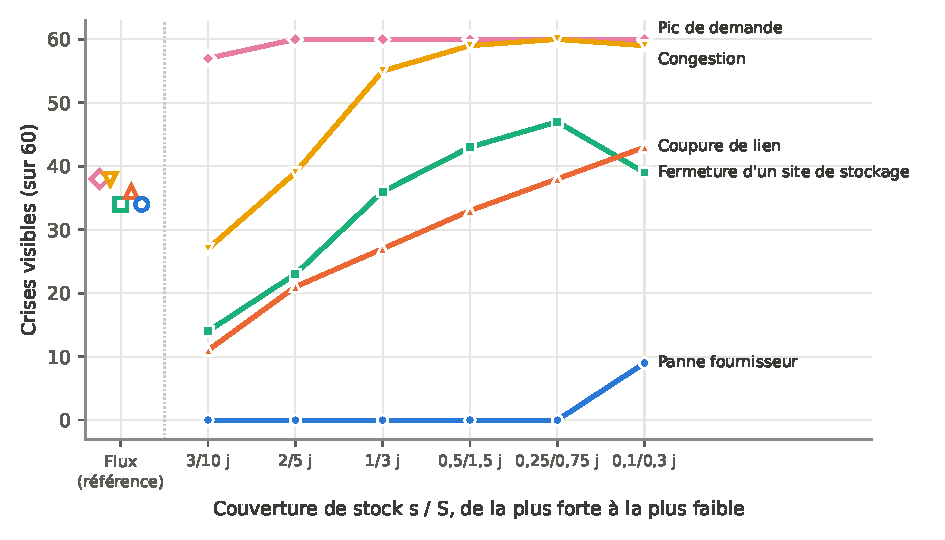
\includegraphics[width=0.75\textwidth]{figures/Fig8_couverture_stock.pdf}
\captionof{figure}{Nombre de crises visibles sur 60 selon la couverture de stock, par nature de perturbation (réseau ISOMORPH, sans réaction). Les symboles creux, à gauche, donnent la référence de la représentation par flux.}\label{fig:d8}
\end{center}

Pour les ruptures de distribution, coupure de lien, fermeture d'un site de stockage et congestion, la couverture agit comme un levier de robustesse progressif : plus elle est faible, plus les crises visibles sont nombreuses, de 11 à 43 sur 60 pour une coupure de lien et de 27 à 59 pour une congestion. La frontière entre robustesse et résilience évoquée en section~S4.3 se déplace donc de manière contrôlée avec le niveau de stock. Les pannes fournisseur sont au contraire absorbées dès que la couverture atteint un quart de jour, y compris pour des pannes de 15 à 60 jours à la couverture par défaut : la calibration de la demande borne le manque à servir pendant une panne, que quelques jours de stock suffisent à compenser. Enfin, le pic de demande est mieux absorbé sans stocks qu'avec : dans la représentation par flux, toute marge de capacité sert instantanément le surcroît de demande, alors qu'avec des délais, ce surcroît doit d'abord être prélevé sur des stocks dimensionnés sur le débit nominal, que le recomplètement ne reconstitue qu'après un délai.

La couverture de stock n'est donc pas un levier universel de résilience. Elle protège contre les pertes de capacité de distribution, est presque superflue contre une défaillance amont de faible ampleur et ne protège pas contre un choc de demande, qui appelle des leviers de capacité ou de demande. Ces résultats, obtenus sans réaction du responsable des opérations et à couverture uniforme, n'épuisent pas la question. L'interaction entre couverture et politique de gestion reste à étudier.

\begin{table}[htbp]
\caption{Crises produisant une baisse de service visible, sur 60, selon la couverture de stock (réseau ISOMORPH, sans réaction).}
\label{tab:S4}
\footnotesize
\begin{tabularx}{\textwidth}{@{}LLLLLLLL@{}}
\toprule
\textbf{Nature} & \textbf{Flux} & \textbf{3 / 10 j} & \textbf{2 / 5 j} & \textbf{1 / 3 j} & \textbf{0,5 / 1,5 j} & \textbf{0,25 / 0,75 j} & \textbf{0,1 / 0,3 j} \\
\midrule
Panne fournisseur & 34 & 0 & 0 & 0 & 0 & 0 & 9 \\
Coupure de lien & 36 & 11 & 21 & 27 & 33 & 38 & 43 \\
Fermeture d'un site de stockage & 34 & 14 & 23 & 36 & 43 & 47 & 39 \\
Pic de demande & 38 & 57 & 60 & 60 & 60 & 60 & 60 \\
Congestion & 38 & 27 & 39 & 55 & 59 & 60 & 59 \\
\bottomrule
\end{tabularx}
\end{table}

\subsection{Lecture économique détaillée et coût de la sur-réaction}
\label{sec:S6.5}

La politique réactive est à la fois la plus efficace et la plus rentable par levier : chacun de ses leviers préserve en moyenne 6 630 unités, soit environ un tiers de journée de demande. Pour une marge de 10 euros par unité, elle reste rentable tant qu'un levier coûte moins de 66 000 euros par crise. La politique prudente est au contraire économiquement dominée : elle engage plus des deux tiers des leviers de la politique réactive pour un quart de ses gains. Chaque levier qu'elle ajoute à la politique tardive ne préserve que 790 unités. Le coût d'une politique tient donc moins au nombre de leviers qu'à leur moment d'engagement : engagés tôt, ils évitent l'allongement de la crise ; engagés tard ou dans le mauvais ordre, ils arrivent quand l'essentiel de la perte est consommé. La rentabilité dépend aussi de la nature du choc : le seuil de la politique réactive atteint 13 100 unités par levier pour une panne fournisseur, mais seulement 2 300 pour une congestion, que des leviers globaux atténuent mal. Le seuil élevé de la politique tardive appelle une réserve : ses gains viennent surtout des leviers de demande, en particulier du report de la demande non critique, qui relève le taux de service mesuré en différant des ventes plutôt qu'en les préservant. Une partie de ces gains est donc reportée sur la période suivante. Son seuil de rentabilité est probablement surestimé.

La figure~7 du manuscrit en tire la conséquence pour le choix d'une politique. Parmi les politiques fixes, la réactivité est optimale tant que le coût d'un levier reste sous le seuil de 6 630 unités de marge ; au-delà, mieux vaut ne pas réagir. Les politiques prudente et tardive ne sont jamais le meilleur choix. La courbe noire en tirets retient, pour chaque crise et chaque coût de levier, la politique au meilleur bénéfice, puis en fait la moyenne sur les 2 000 crises. Ce choix est fait a posteriori, comme si l'issue de chaque politique était connue d'avance : la courbe constitue donc une limite haute de ce qu'une préconisation adaptée à la crise peut rapporter, dont le réseau bayésien, qui ne connaît la crise que partiellement, ne capte qu'une partie. Cette limite haute conserve un bénéfice positif bien au-delà du seuil de la politique réactive, parce que pour certaines crises la politique tardive ou l'absence de réaction suffisent. Pour un levier valant 5 000 unités de marge, le choix adapté porterait le bénéfice moyen de 4 560 à 8 350 unités par crise, soit 83~\% de plus que la meilleure politique fixe ; pour un levier plus coûteux, il resterait le seul à dégager un gain. La préconisation du réseau bayésien vise précisément cette valeur, en repérant, à partir de ce que l'on sait d'une crise, les cas où une politique plus sobre suffit.

Deux lots complémentaires, aux réglages du lot principal, mesurent le coût de la sur-réaction : 400 scénarios sans perturbation perceptible et 300 perturbations mineures (sévérité de 0,1 à 0,3, durée de 1 à 3 jours). Sans perturbation, aucun profil n'engage de levier, car la détection, fondée sur le taux de service lissé, ne se déclenche pas sur les seules fluctuations de la demande. Face à une perturbation mineure, en revanche, le profil réactif engage au moins un levier dans 32~\% des cas, contre 4~\% pour le profil prudent et aucun pour le profil tardif, pour ne réduire les ventes perdues que de 2 335 à 2 260 unités par crise. Chaque levier y préserve environ 230 unités, près de trente fois moins que sur l'ensemble des crises de la base principale. La sensibilité du profil réactif a donc un coût réel face aux chocs mineurs, pour l'essentiel des pics de demande et des congestions : elle ne se justifie que si l'on sait distinguer un choc mineur d'une crise sévère, ce que vise le pronostic du réseau bayésien.

\section{Reproductibilité des figures et des tableaux}
\label{sec:S7}
\sloppy


Cette partie indique, pour chaque figure tirée des données, comment la reproduire à partir des fichiers déposés avec l'article et de l'application Isomorph-Reborn.

\subsection*{Réseau ISOMORPH (figure~\ref{fig:d2})}

Dans l'application Isomorph-Reborn, fournie avec l'article, ouvrir l'onglet « Générateur de scénarios » ; dans la section « Réseau », en tête de l'onglet, choisir « Réseau ISOMORPH » pour afficher le schéma par échelons de la figure~\ref{fig:d2}. La description du réseau, avec ses capacités et ses délais de trajet, est contenue dans le fichier \texttt{reseau\_isomorph-originel.json}.

\subsection*{Crise S0366 sous les quatre politiques (figure~2 du manuscrit)}

Dans l'onglet « Générateur de scénarios » d'Isomorph-Reborn, charger le fichier d'hypothèses \texttt{hypotheses\_lot} \texttt{\_A\_isomorph\_tension75.json} (réseau ISOMORPH, représentation par flux, niveau de tension 75, 2 000 scénarios, graine 42) et lancer la génération. Les trajectoires journalières sont exportées dans le fichier \texttt{ip\_timeseries.csv} (colonnes \texttt{scenario\_id}, \texttt{branch\_id}, \texttt{day\_rel} et \texttt{ip}) ; la figure~2 du manuscrit en reprend les quatre versions du scénario S0366. Les jours de détection proviennent de la base d'apprentissage exportée pour le même lot.

\subsection*{Ajustement de la crise S0366 (figure~\ref{fig:d4})}

Les paramètres ajustés de chaque version de crise sont exportés par Isomorph-Reborn (onglet « Ajustement par lot ») dans le fichier \texttt{resilience\_ip.csv} (colonnes \texttt{k}, \texttt{q}, \texttt{h}, \texttt{g}, \texttt{d}, \texttt{alpha}, \texttt{beta}, \texttt{r2}, puis les six indicateurs). La courbe tracée est l'équation (2) du manuscrit évaluée avec les paramètres de la ligne S0366, version \texttt{none}, superposée à la trajectoire du fichier \texttt{ip\_timeseries.csv}. Dans l'application, cette crise est la courbe n° 1461 sur 8 000 : le compteur numérote les versions de crise, à raison de quatre par scénario, et non les scénarios.

\subsection*{Apprentissage du réseau bayésien (figure~4 du manuscrit)}

Dans BayesArtist, importer la base \texttt{bayesartist\_apprentissage\_lotA.csv} (6 400 versions de crise, 20 variables) et les contraintes \texttt{bayesartist\_contraintes\_isomorph.json} (155 arcs interdits, quatre parents au plus), puis lancer l'apprentissage par recherche gloutonne (\textit{Greedy Hill Climbing}) au score BIC avec lissage de Laplace. Le réseau appris s'exporte au format \texttt{.bif} ; la figure est tracée à partir de ce fichier. BayesArtist n'étant pas diffusé, le même apprentissage peut être conduit avec tout logiciel de réseaux bayésiens qui apprend à partir d'un fichier CSV et accepte des arcs interdits (voir la déclaration de disponibilité des données du manuscrit).

\subsection*{Pronostic de l'étude de cas (figure~\ref{fig:d7})}

Dans BayesArtist, en mode inférence sur le réseau de la figure~4 du manuscrit, poser les évidences nature = \texttt{fermeture\_entrepot}, cible = \texttt{passage\_oblige} et durée = \texttt{fort}, puis fixer successivement le profil à \texttt{none}, \texttt{tardif}, \texttt{prudent} et \texttt{reactif}, et lire à chaque fois la distribution du nœud IPC.

\subsection*{Carte de préconisation (figure~5 du manuscrit)}

Dans BayesArtist, sur le réseau de la figure~4 du manuscrit, poser les évidences nature, cible et durée correspondant à un contexte de la carte, ainsi que IPC = \texttt{faible}, puis lire la distribution du nœud profil. La carte est calculée par inférence exacte sur le réseau exporté au format \texttt{.bif} ; BayesArtist, dont l'inférence est approchée, donne les mêmes valeurs à 0,01 près (par exemple 0,06, 0,08, 0,10 et 0,76 pour la fermeture longue d'un point de passage obligé).

\subsection*{Lecture économique (tableau~9 et figure~6 du manuscrit)}

Les ventes perdues sont calculées à partir du fichier \texttt{ip\_timeseries.csv} du lot A, comme la somme de $1 - \mathrm{IP}(t)$ sur les 60 jours suivant le choc multipliée par la demande de référence ; le nombre de leviers engagés et la demande de référence proviennent de la base d'apprentissage exportée pour le même lot (colonnes \texttt{nb\_decisions} et \texttt{base\_demand}).


\bibliographystyle{cas-model2-names}
\bibliography{references}

\end{document}
